\documentclass[11pt, a4paper]{article}
\sloppy %prevents text from going over the right margin
% \usepackage[T1]{fontenc}
\usepackage[utf8]{inputenc}
\usepackage{listings}
\usepackage[margin=1.0in]{geometry}
\usepackage{color}
\usepackage{graphicx}
\usepackage{tabularx}
\usepackage{url}
\usepackage[normalem]{ulem} 
\usepackage{enumitem}
\usepackage{hyperref}
\usepackage{fancyhdr} %Package to configure headings and footer
\usepackage{lastpage}
\usepackage{gensymb}
\usepackage[version=3]{mhchem}
\usepackage[ngerman]{babel}
\setlength\parindent{0pt}

\newcommand{\VARtitle}{NW2}
\newcommand{\VARauthor}{Janeczek}

\title{Koaxialkabel und Glasfaserkabel \\ \VARtitle}
\author{\VARauthor}
\date{\today{}, Vienna}

% header
\pagestyle{fancy}
\fancyhead[L]{\today}
\fancyhead[R]{\VARtitle}

%footer
\fancyfoot[L]{\VARauthor}
\fancyfoot[C]{5AHITT}
\fancyfoot[R]{Page \thepage/\pageref{LastPage}}


\begin{document}

\lstset{ %
  backgroundcolor=\color{white},   % choose the background color; you must add \usepackage{color} or \usepackage{xcolor}
  basicstyle=\footnotesize,        % the size of the fonts that are used for the code
  breakatwhitespace=false,         % sets if automatic breaks should only happen at whitespace
  breaklines=true,                 % sets automatic line breaking
  captionpos=b,                    % sets the caption-position to bottom
% commentstyle=\color{mygreen},    % comment style
  deletekeywords={...},            % if you want to delete keywords from the given language
  escapeinside={\%*}{*)},          % if you want to add LaTeX within your code
  extendedchars=false,              % lets you use non-ASCII characters; for 8-bits encodings only, does not work with UTF-8
% frame=single,                    % adds a frame around the code
  keepspaces=true,                 % keeps spaces in text, useful for keeping indentation of code (possibly needs columns=flexible)
% keywordstyle=\color{blue},       % keyword style
% language=bash,                   % the language of the code
  morekeywords={*,...},            % if you want to add more keywords to the set
  numbers=left,                    % where to put the line-numbers; possible values are (none, left, right)
  numbersep=5pt,                   % how far the line-numbers are from the code
  rulecolor=\color{black},         % if not set, the frame-color may be changed on line-breaks within not-black text (e.g. comments (green here))
  showspaces=false,                % show spaces everywhere adding particular underscores; it overrides 'showstringspaces'
  showstringspaces=false,          % underline spaces within strings only
  showtabs=false,                  % show tabs within strings adding particular underscores
  stepnumber=1,                    % the step between two line-numbers. If it's 1, each line will be numbered
  tabsize=2,                       % sets default tabsize to 2 spaces
  title=\lstname                   % show the filename of files included with \lstinputlisting; also try caption instead of title
}


\maketitle
\newpage
\tableofcontents
\newpage


\section{Vorwort}

In diesem Dokument wird eine meiner naturwissenschaftlichen Thematiken ausgearbeitet. Es handelt sich um den Fachbereich der Kommunikationstechnik. Ich werde euch einen wesentlichen Überblick bezüglich dem Aufbau und der Funktionsweise von Koaxial- und Glasfaserkabeln, sowie einer Gegenüberstellung dieser geben.

\section{Koaxialkabel \cite{koaxialkabel} \cite{koaxialkabel-wiki}} 

\subsection{Begriffserklärung}
\textbf{Was ist ein Koaxialkabel?}\\
Unter einem Koaxialkabel oder Koaxialleitungen versteht man Bus- oder Ring-Verkabelungen, die lange Zeit in der Netzwerktechnik eingesetzt wurden. Durchgesetzt haben sich jedoch strukturierte Stern-Verkabelungen auf Basis von Twisted-Pair-Kabel. \\ \\Im Grundlegenden spricht man bei der Verwendung eines Koaxialkabels von elektrischen Signalen/Daten, die meist in Kupferleitungen als Elektronen von Sender zum Empfänger geschickt werden.

\subsection{Aufbau eines Koaxialkabels}
\textbf{Wie ist ein Koaxialkabel aufgebaut?}\\
Der Kern des Koaxialkabels ist der sogenannte Innenleiter (meist eine Kupferader, bzw. ein gut leitendes Metall). Dieser Kern wird von einer Isolationsschicht umhüllt, die meist aus Kunststoff oder ähnlichem besteht. Dem Kabel wird dadurch zusätzliche mechanische Stabilität gegeben.\\ \\ Um der Isolationsschicht herum befindet sich ein Schirmgeflecht als Außenleiter. Wenn nun an diesem Leiter eine Spannung angelegt wird, entsteht das elektrische Feld nur zwischen dem Außen- und Innenleiter. Es tritt also kein Magnetfeld außerhalb des Kabels auf. \\ \\

\begin{figure}[h!]
	\centering
	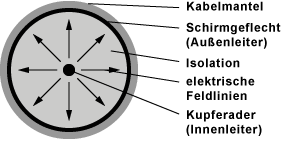
\includegraphics[width=0.6\textwidth]{images/coax-aufbau}
	\caption{Illustration des Aufbaus eines Koaxialkabels \cite{koax-img}}
\end{figure}

\newpage
Der Außenleiter dient als Antenne und schirmt elektromagnetische Strahlen ab. Außerdem
beeinflussen Störungen von außen (Magnetfelder, die von anderen unter Spannung stehenden Kabeln erzeugt werden) den Signalfluss im Innenleiter und aus diesem Grund muss der
Außenleiter an Erde gelegt werden. Somit wird die elektrische Feldverteilung wirksam. Das bereits erwähnte Schirmgeflecht ist eine allseitig geschlossene Hülle, die als elektrische Abschirmung  für das Kabel wirkt.

\subsection{Vorteile gegenüber Twisted-Pair-Kabel}
Ein Twisted-Pair-Kabel ist ein Kabel, bei dem die einzelnen Teilkabeln paarweise miteinander verdrillt wurden. Diese paarweise Verseilung und ein elektrisch leitender Schirm vermindern störende Einflüsse von äußeren magnetischen Wechselfeldern. Ebenso wird das Übersprechen zwischen benachbarten
Adernpaaren innerhalb des Kabels reduziert.\\ \\
\textbf{Welche Vorteile hat das Koaxialkabel gegenüber dem Twisted-Pair-Kabel?}
\begin{itemize}
\item Es können keine Störspannungen durch Influenz in das Kabel gelangen
\item Die im Kabel fließenden Ströme erzeugen keine magnetischen Störfelder.
\end{itemize}

\subsection{Anwendungen des Koaxialkabels}
Das Koaxialkabel wurde häufig als Netzwerkkabel verwendet, heutzutage eher selten, da der Lichtwellenleiter eine wesentlich größere Leistung erbringen kann. \\ \\
Desweiteren finden Koaxialkabel als Antennenkabel oder für die Übertragung von TV und Radio (Rundfunk/Broadcast) Einsatz.

\section{Lichtwellenleiter \cite{lwl} \cite{lwl-wiki}}

\subsection{Begriffserklärung}
\textbf{Was ist ein Lichtwellenleiter?}\\
Unter einem Lichtwellenleiter oder auch als LWL/Glasfaser bekannt, versteht man alle licht-leitenden Leitungen, die entweder aus Glas-, Quarz- oder Kunststofffasern bestehen. Bei dem Koaxialkabel werden Daten als Elektronen gesendet, bei dem Lichtwellenleiter hingegen,
übernehmen die Photonen (Lichtteilchen) diese Aufgabe. \\ \\
Durch Lichtwellenleiter können optische Signale mit dem Einsatz von wenigen Verstärkern große Entfernungen überbrücken. Trotz weiter Strecken ist eine hohe Bandbreite aufgrund von mehreren, gleichzeitig gesendeten Lichtwellen mit unterschiedlicher Wellenlänge möglich. Das macht den Lichtwellenteiler zum Übertragungsmedium der Gegenwart und Zukunft. Da kommt ein Kupferkabel oder Funksystem einfach nicht heran. \\ \\
Die Glasfaser zum Beispiel ist ein solcher Lichtwellenteiler, dessen Fasern aus deem Grundstoff Glas bestehen.

\newpage
\subsubsection{Prinzip der Übertragung}
Das zu sendende Signal wird mittels Analog-Digital-Wandlung in ein elektrisches Signal umgewandelt,
welches dann noch von einer Treiberstufe verstärkt wird. Damit das Prinzip des Lichtwellenleiters angewandet werden kann, müssen zunächst die elektrischen Signale in optische Signale umgewandelt werden. Dazu dienen spezielle Leuchtdioden oder Laserdioden. \\ \\
Nach diesem Vorgang wird das Lichtsignal in den Lichtwellenleiter eingespeist. Am anderen Ende des LWLs werden die Lichtimpulse wieder in elektrische Signale umgewandelt. Dazu wird meist ein Fototransistor verwendet. Diese elektrischen Signale müssen nun wieder Digital-Analog umgewandelt werden. Die Daten werden dann in analoger Form verstärkt und an den Empfänger übergeben.

\begin{figure}[h!]
	\centering
	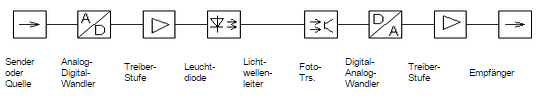
\includegraphics[width=1.0\textwidth]{images/lwl2}
	\caption{Das Prinzip der Übertragung \cite{lwl-uebertragung-img}}
\end{figure}

\subsubsection{Aufbau eines Lichtwellenleiters}
LWL aus Kunststoff haben meist einen Durchmesser von etwa 0,1mm und sind äußerst flexibel aber
auch empfindlich. Der Faserkern (Kernglas) ist der zentrale Bereich eines Lichtwellenleiters, der zur
Wellenführung des Lichts dient. Dieser Kern  besteht aus einem Material mit einem höhren Brechungsindex
als der darüberliegende Mantel. An den Wänden im Inneren des LWLs findet eine Totalreflexion statt,
sodass der Lichtstrahl nahezu verlustfrei um jede Ecke geleitet wird. 

\begin{figure}[h!]
	\centering
	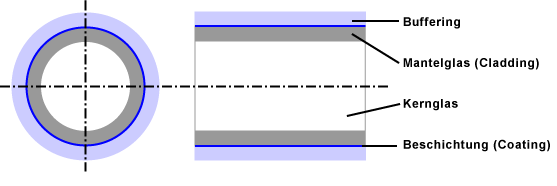
\includegraphics[width=1.0\textwidth]{images/lwl}
	\caption{Illustration des Aufbaus eines Lichtwellenleiters \cite{lwl-img}}
\end{figure}

Das Mantelglas hat reflektierende Eigenschaften (transparentes Material), ist nicht leitend und hat keine metallischen
Anteile. Buffering nennt man das Schutzmaterial, das auf dem Coating aufextrudiert ist. Es schützt
das Kabel vor Umwelteinflüssen.

\subsubsection{Vorteile gegenüber Kupferkabel}
Der Einsatz von LWLs wird im wesentlichen durch diese Vorteile unterstrichen:
\begin{itemize}
\item Lichtwellenleiter können beliebig mit anderen Versorgungsleitungen parallel verlegt werden, es
wirken keine elektromagnetischen Störeinflüsse.
\item Wegen der optischen Übertragung existieren keine Störstrahlungen oder Masseprobleme
\item Entfernungsbedingte Verluste durch Induktivitäten, Kapazitäten und Widerständen treten nicht
auf
\item Nahezu Frequenz-unabhängige Leitungsdämpfung der Signale
\item Übertragungsraten sind durch mehrere Trägerwellen mit unterschiedlichen Wellenlängen
(Farbspektrum) fast unbegrenzt erweiterbar, daher auch die hohe Bandbreite
\end{itemize}
Diese genannten Vorteile bringen aber auch einige Nachteile mit sich. Lichtwellenteiler sich an sich wesentlich teurer als Kupferleitungen. Die Kosten für Material und Montage sind um einiges höher. Kurz zusammengefasst: Der Einsatz von Glasfaserkabeln eignet sich besonders gut für große Strecken und schlägt somit die Kupferleitungen im Kampf der Kommunikationstechnik. \\ \\
Betätigt man nun den Lichtschalter, geht das Licht für uns in Lichtgeschwindigkeit an. \\
Die Ladungsträger können sich nicht mit Lichtgeschwindigkeit bewegen, da diese eine Masse besitzen. Eine Masse kann niemals auf Lichtgeschwindigkeit gebracht werden. Wenn man den Lichtschalter betätigen würde, würde die Masse der Elektronen ins Unendliche schreiten. Die Elektronen breiten sich wiederrum mit der Lichtgeschwindigkeit aus.
\newpage
\nocite{*}
\bibliographystyle{plain}
\bibliography{bibliography}{}

\end{document}